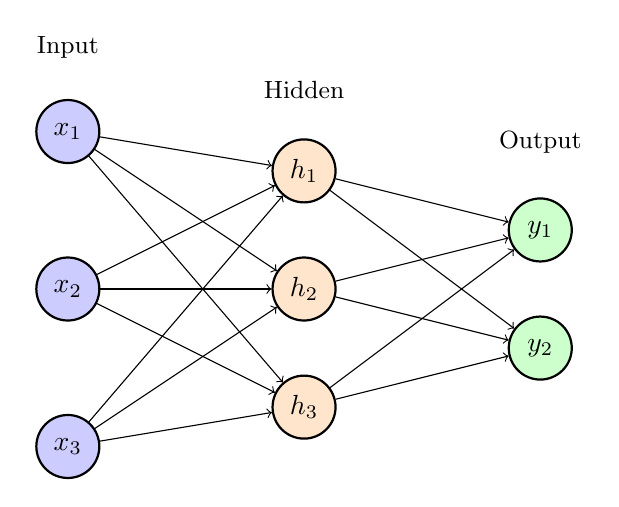
\begin{tikzpicture}[
    node distance=1.5cm,
    neuron/.style={circle, draw, minimum size=0.8cm, thick},
    input/.style={neuron, fill=blue!20},
    hidden/.style={neuron, fill=orange!20},
    output/.style={neuron, fill=green!20},
]
    % Input layer
    \node[input] (i1) at (0,2) {$x_1$};
    \node[input] (i2) at (0,0) {$x_2$};
    \node[input] (i3) at (0,-2) {$x_3$};

    % Hidden layer
    \node[hidden] (h1) at (3,1.5) {$h_1$};
    \node[hidden] (h2) at (3,0) {$h_2$};
    \node[hidden] (h3) at (3,-1.5) {$h_3$};

    % Output layer
    \node[output] (o1) at (6,0.75) {$y_1$};
    \node[output] (o2) at (6,-0.75) {$y_2$};

    % Connections input -> hidden
    \foreach \i in {1,2,3}
        \foreach \h in {1,2,3}
            \draw[->] (i\i) -- (h\h);

    % Connections hidden -> output
    \foreach \h in {1,2,3}
        \foreach \o in {1,2}
            \draw[->] (h\h) -- (o\o);

    % Labels
    \node[above=0.3cm] at (0,2.5) {\small Input};
    \node[above=0.3cm] at (3,2) {\small Hidden};
    \node[above=0.3cm] at (6,1.3) {\small Output};
\end{tikzpicture}
